\documentclass[10pt,a4paper,notitlepage]{scrreprt}
\usepackage[utf8]{inputenc}
\usepackage{amsmath}
\usepackage{amsfonts}
\usepackage{amssymb}
\usepackage{graphicx}
\usepackage{xcolor}
\usepackage{geometry}
\usepackage{ngerman}
\usepackage{textcomp}
\usepackage[autostyle=true,german=quotes]{csquotes}
\usepackage{multirow}
\usepackage{setspace}

\begin{document}
	\newgeometry{bottom=3cm}
	
	\pagestyle{headings}
	\onehalfspacing
	\title{Dokumentation \\ Komplexpraktikum Medieninformatik \\ Multimediatechnologie}
	\author{\textbf{Gruppe 2} \\Gruppenleiter: Alexandra Krien \\  Georg Eckert \\ Stephanie Sara Groß \\ Philipp Roscher \\ Ehemals: Nathalie Blasberg   }
	\maketitle
	\tableofcontents


	\chapter{Einleitung}

	Wir sind Gruppe 2, die im Rahmen des Komplexpraktikums Medieninformatik, Teilgebiet Multimediatechnologie, eine Spielsoftware entwickelt.\\ 
	Unsere Gruppenmitglieder sind dem Titelblatt zu entnehmen.\\
	Aufgabe des Komplexpraktikums ist es, in einer Gruppe von fünf Studenten eine Software zu entwickeln.\\
	Spezifisch soll es sich dabei um ein Multiplayer-Spiel handeln, welches das Prinzip der \enquote{Game Orchestration} einbezieht.\\
	Bei diesem Konzept handelt es sich um eine Form der Rollenverteilung innerhalb eines Spiels.\\
	Dabei übernimmt einer der Spieler die Rolle des Game Masters der in besonderer Art und Weise Einfluss auf das Spielgeschehen nehmen kann.\\
	Dies kann verschiedene Auswirkungen auf die Position des Game Masters gegenüber den weiteren Spielern haben. So kann er sowohl unterstützend, als auch als Antagonist auftreten.\\
	In unserem Spielkonzept entschieden wir uns für die Rolle des Antagonisten.\\
	Weitere Vorgaben beschränken sich lediglich auf das Framework libGDX, sowie die Nutzung einer  Netzwerkkommunikation. Genauer gehen wir darauf im Bereich 'Technologie' ein.\\

	\chapter{Konzept}

		\section{Story}
		In einem Labyrinth tief unter der Erde, lebt ein Drache und beschützt dort seit Jahren einen Schatz. Kämpfer aus dem ganzen Land reisen an um sich den Schatz unter den Nagel zu reißen. Erst wenn sie den Drachen und andere Widersacher besiegt und alle Schlüsselteile gesammelt haben, können sie den Schatz ergattern und aus dem Labyrinth entkommen.\\
		
		\section{Setting}
		Es nehmen 5 Spieler teil. Dafür werden zwei Gruppen und ein Game Master durch Zufall entschieden.\\
		Der Game Master ist der Drache und muss den Schatz vor den anderen zwei Gruppen beschützen. Dafür hat er verschiedene Fähigkeiten: Als Herrscher des Labyrinths hat er Überblick über alle Kammern, kann geheime Pfade nutzen und Monster in dem Kampf schicken. Da er viel strategischer handelt als die anderen Spieler und weniger Lebenspunkte hat, legt er mehr Wert auf seine Verteidigung.\\
		Die zwei Teams bestehen aus jeweils zwei Spielern. Nachdem die Aufteilung durch Zufall entschieden wurde, können die Teilnehmer ihre Spielfigur auswählen. Je nach Klasse liegen unterschiedliche Angriffe vor.\\
		Nach der Auswahl fängt das Spiel im Labyrinth an. \\
		Dieses wird zufällig generiert und ist somit bei jedem neuen Spielstart anders. Die Spielr starten entsprechend der Teamaufteilung in drei verschiedenen Spawnräumen. Ziel ist die Schatzkammer in der Mitte des Labyrinthes.\\
		
		\section{Rollenverteilung und Charaktere}
		In unserem Spiel existiert eine Vielzahl an spielbaren Klassen.\\

			\subsection{Der Drache} 
			Der Beschützer des Schatzes und der Herr des Labyrinths. Er agiert als Game Master. Seine Strategie ist die Verteidigung. Angreifen kann er durch das Speien von Feuer. Zusätzlich kann er auch Monster spawnen.\\
			
			\subsection{Fernkampf}

				\subsubsection{Schamane}
				Der Schamane ist ein Magier, sein Angriff ist das Schießen von magischen Sphären.\\
				
				\subsubsection{Bogenschütze}
				Der Bogenschütze greift klassisch mit Pfeilen an.\\

			\subsection{Mittelfernkampf}

				\subsubsection{Ninja}
				Der Ninja greift mit dem Werfen von Shuriken an.\\
				
				\subsubsection{Hexe}
				Die Hexe ist ein Magier, ihr Angriff ist das Schießen von magischen Sphären.\\

			\subsection{Nahkampf}

				\subsubsection{Schwertkämpfer}
				Der Schwertkämpfer kämpft mit dem Schwert.\\
				
				\subsubsection{Kämpfer}
				Der Kämpfer kämpft mit dem nackten Fäusten.\\

		\section{Spielende}
		Ziel ist das Erbeuten des Schatzes. Dazu müssen zunächst alle drei Schlüsselfragmente ergattert werden. Zu Beginn des Spiels erhält jedes Team ein Fragment. Stirbt der Schlüsselträger eines Teams, wird das Fragment abgeworfen und kann eingesammelt werden. Der getötete Spieler respawnt nach einigen Sekunden wieder am Startpunkt. Ist ein Team im Besitz aller drei Fragmente, muss danach noch die Schatzkammer bertreten werden. Erst danach kann das Spiel beendet werden.\\

		\section{Design}
		Bei dem Spiel handelt es sich um ein dungeonbasiertes Top Down Game im Pixellook. Die Sprites für das Labyrinth sind Open Source, mit einigen eigenen Erweiterungen. Alle Charakter und UI Elemente wurden von uns entworfen.\\

			\subsection{Welt}
				\begin{center}
						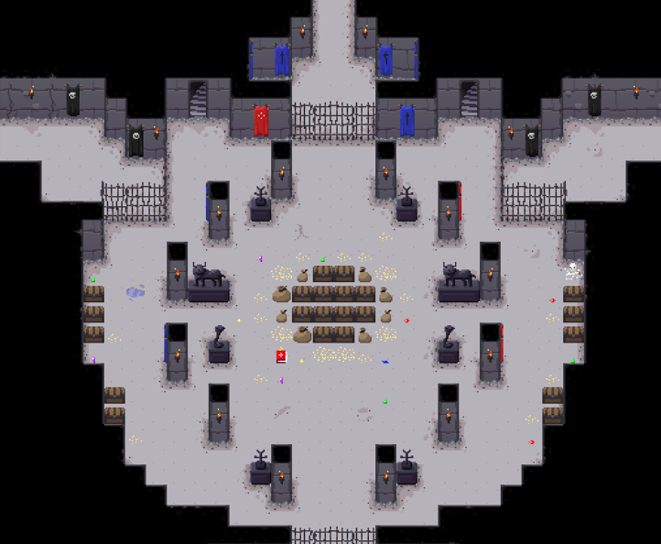
\includegraphics[scale=0.8]{maze.png}\\
					Die Schatzkammer\\\
			
					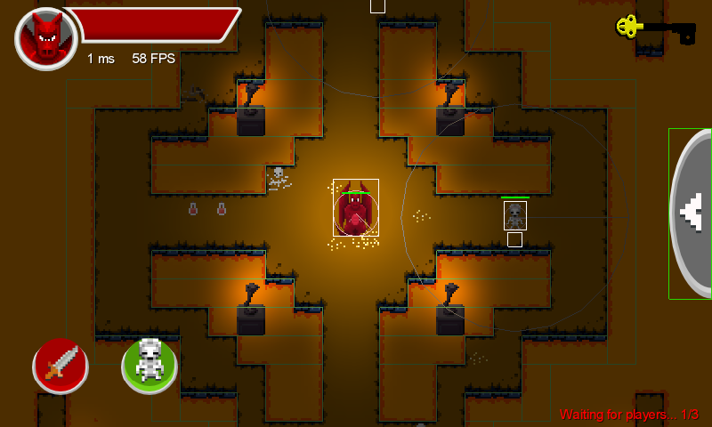
\includegraphics[scale=0.8]{mazewithui.png}\\
					Spawnroom mit überlappendem Interface\\
				\end{center}
			
			\subsection{Spielfiguren}
				\begin{center}
					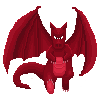
\includegraphics[scale=2]{Dragon}\\
					Der Drache\\
						
					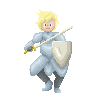
\includegraphics[scale=2]{Knight}
					
\includegraphics[scale=2]{Fighter}\\
					Der Schwertkämpfer und der Faustkämpfer\\
					
					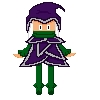
\includegraphics[scale=2]{Witch}
					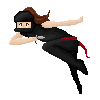
\includegraphics[scale=3.5]{Ninja}\\
					Die Hexe und der Ninja\\
					
					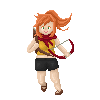
\includegraphics[scale=2]{Archer}
					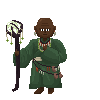
\includegraphics[scale=2]{Shaman}\\
					Der Bogenschütze und der Schamane\\
				\end{center}
			
		\section{Technologie und Steuerung}
		Das Spiel ist sowohl auf PC, als auch Android spielbar. Die Oberfläche unterschiedet sich dabei nicht. Die Steuerung hingegen ist entsprechend angepasst. Gespielt wird auf dem PC mit Maus und einigen Tasten, auf Android komplett über Touch.\\
		Voraussetzung für das Spiel ist ein Endgerät mit respektive Windows 7 oder höher, Linux mit Kernel 3.16 oder höher, Android 4 oder höher. Das Gerät muss Open GL unterstützen und netzwerkfähig sein. Oracle Java muss mindestens in Version 1.6 installiert sein. Für ein gutes Spielerlebnis werden mindestens Geräte mit 2 Prozessorkernen > 1GHz und einer Bildschirmauflösung von 480x800 Bildpunkten empfohlen.\\
	
	\chapter{Implementierung}
		\section{Planung und Entwicklung}
			\subsection{ Prototypen}
			Im Prototypen entschieden wir uns zunächst für getrennte Anwendungen. So entstanden individuell ein Prototyp für die Bewegung der Spielfigur, die Game Master Fähigkeiten, die Generierung eines simplen zufälligen Labyrinthes und das Netzwerk.\\
			Im Anschluss führten wir die einzelnen Prototypen zusammen und arbeiteten an einer gemeinsamen Anwendung weiter.\\
			
			\subsection{Alpha}
			
			Mit der Alpha wurde unser Spiel grundsätzlich durchspielbar. Das Labyrinth wurde erweitert und generierte sich zufällig aus einer Auswahl von 10 Labyrinth-teilen, den Spawnräumen und einer Schatzkammer. Auch ein simples Inventar ist nun vorhanden um Schlüsselteile sammeln zu können. Entsprechend können Spieler jetzt sobald sie alle 3 Schlüsselteile haben die Schatzkammer betreten und das Spiel gewinnen.\\
			Der Game Master konnte nun durch für ihn reservierte Pfade im Labyrinth gehen, als erste asymmetrische Implementierung im gemeinsamen Projekt.\\
			Außerdem wurde ein Spielerstatus ergänzt, durch den Spieler und Game Master nun sterben und respawnen kann.\\
			
			\subsection{Beta}
			
			Die größte Veränderung in der Entwicklung der Beta war, dass wir viel vom Client auf den Server ausgelagert haben. So läuft nun die komplette Physik, Monster und Items auf dem Server.\\
			Der Spielbeginn wurde verbessert, so dass die Spieler nun auswählen können welche Klasse sie Spielen möchten. Außerdem stehen nun erstmals alle 6 Klassen zur Auswahl. Im Anschluss muss auch nicht mehr auf dem Titelbildschirm gewartet werden bis genug Spieler beigetreten sind. Stattdessen ist man nun im jeweiligem Spawnraum eingeschlossen und kann sich schonmal mit der Steuerung vertraut machen.\\
			Der Game Master kann nun kleine Gruppen von Monstern spawnen.\\
			Monster haben nun eine rudimentäre KI, durch die sie Spielern folgen, sobald sie in einem bestimmten Radius zum Spieler sind.\\
			Ein optisches Feedback wenn man Schaden nimmt wurde ebenfalls ergänzt.\\
			Das Labyrinth hat nun genug Teile, aus denen es sich aufbaut, um Duplikate zu vermeiden.\\
			Die Schatzkammer öffnet sich nun für beide Teammitglieder, dank eines gemeinsamen Schlüssel-Inventars.\\
			
			\subsection{Endprodukt}
			
			Das abschließende Endprodukt enthält größtenteils Änderungen die das Spielerlebnis verbessern. So gibt es nun eine Minimap, die sich nach und nach mit dem Erkunden des Labyrinths aufdeckt, und einem die Position des Teammitglieds zeigt.\\
			Das Inventarsystem wurde um Heiltränke erweitert, die nun sowohl im Labyrinth zufällig gefunden werden, als auch von besiegten Monstern fallengelassen werden können. Außerdem kann man im Inventar nun auch zwischen Nah- und Fernkampfwaffen wechseln.\\
			Die Monster-KI wurde verbessert und sie können nun Spieler verfolgen und angreifen.\\
			Die Balance zwischen Spielern und Monstern wurde verbessert, als auch zwischen Game Master und Spielern.\\

	\section{Entwurfsentscheidungen}

		\subsubsection{Das Labyrinth und die Minimap}
		
		Das Labyrinth wird mit Start des Servers generiert und an die Clients übergeben. Grundlage bilden vorgefertigte TiledMaps im Format 32 * 32 Kacheln mit 32 * 32 Pixeln pro Kachel. In der Generierung werden die vorgefertigten Teile zufällig aneinander gesetzt, die Spawnräume und Schatzkammer platziert und anschließend als eine Map gespeichert. Das Labyrinth ist dabei duplikatsfrei.\\
		An das Labyrinth geknüpft ist die Minimap, sie wird direkt danach erzeugt und als eine Anordnung von Images in Box2D dargestellt. Die Verwaltung von Standorten und aufgedeckten Teilen des Labyrinths übernimmt jeder Client separat.\\
		
		\subsubsection{Charakter}
		
		Die Charaktere sind grundlegend in Game Master und Teams gegliedert. Der Game Master hat dabei nur den Drachen zur Auswahl, wohingegen die Spieler zwischen den 6 Klassen, die im Konzept erklärt wurden, wählen können. Es ist dabei möglich Klassen mehrfach zu belegen.\\
		Die Charakterwahl findet zwar Client-seitig statt, wird aber kontinuierlich mit dem Server synchronisiert, da dort alle Berechnungen (Position, HP, etc.) stattfinden. dadurch sollen eventuelle Manipulationen durch den Client vermieden werden.\\
		Die Charaktererstellung ist auf einem Entity Component System aufgebaut. So entspricht jeder individuelle Character einer Entität mit verschiedenen Komponenten, wie Waffe, Sensorbody, Position, TeamID und Inventar.\\
		
		\subsubsection{Kampfsystem} 
		TODO
		
		\subsubsection{Netzwerkkommunikation}
		
		Das Spiel basiert auf einem Server-Client-System, wobei ein Server sowohl als Standalone-Version als auch aus dem Spiel heraus gestartet werden kann. Das Verbinden ist derzeit nur per IP möglich, eine zentrale Serverliste oder ein automatisches Matchmaking gibt es nicht.\\
		Fast die komplette Spiellogik läuft auf dem Server, wodurch eine spielerseitige Manipulation von Daten, z.B. in Form von Cheats, ausgeschlossen wird. Der Server überträgt relevante Daten per TCP und UDP an den Client. Allerdings gibt es noch kein System zur Lagkompensation und aus Gründen der Flüssigkeit läuft die Bewegung der Spieler noch komplett auf den Clients. An einigen Stellen kommt es hierdurch vor allem bei schlechteren Netzwerkbedingungen zu entsprechenden Problemen, die mit komplexeren Systemen wie bspw. Movement Prediction sicherlich noch gelöst werden können.\\
		
		\subsubsection{Itemsystem}
		
		Das Itemsystem baut ebenfalls auf dem Entity Component System auf. Bei den Items wird hier grundlegend zwischen Waffen, Tränken und Schlüsselteilen unterschieden. Dabei sind die Schlüsselteile zusätzlich an die TeamID gebunden, damit beide Teammitglieder im Interface sehen, wie viele Schlüssel sie besitzen, aber auch damit sie gemeinsam die Schatzkammer betreten können.\\
		Jeder Spieler hat zum Spielbeginn eine festgelegt Auswahl an Tränken und Waffen. (Jeweils einen Klassen-spezifischen Angriff und eine einfache Faust für den Nahkampf). Im Laufe des Spiels können weitere Tränke aufgenommen werden.\\
		Es sollte auch bessere Waffen zu finden geben, zur Implementierung davon ist es aus Zeitgründen jedoch nicht gekommen.\\
		
		\subsubsection{Interface}
		
		Das Interface wurde mit Hilfe von Box2D umgesetzt. Wir nutzen dabei die enthaltenen Button- und Tabellen-Funktionen. Das Startmenü als auch die Charakterauswahl wurden dabei möglichst simpel gehalten.\\
		Während des Spiels ist das Interface ein Overlay über dem eigentlichen Spielgeschehen. Angriffs-Buttons, eine Toolbar um das Menü zu öffnen und Informations-Overlays zu HP und Schlüsselanzahl sind an den Rändern des Bildschirms platziert. So hat dier Spieler alle wichtigen Informationen auf einen Blick ohne dabei zu sehr von eigentlichem Spielgeschehen abgelenkt zu werden.\\
		Das geöffnete Inventar befindet sich mittig und verdeckt den Großteil des Bildes, es ist jedoch auch so möglich sich weiter zu bewegen und alle anderen Buttons zu erreichen. Das Inventar selbst besteht aus weiteren Buttons. Im oberen Bereich kann man zwischen zwei Waffen (der Faust und der Klassen-spezifischen Waffe) wählen. Im Zentrum befinden sich Heiltränke, die durch einfaches anklicken eingesetzt werden können. unten rechts ist ein Button über den die Mini-Map geöffnet werden kann.\\
		Außerdem bleibt am rechten Rand des Bildschirms die Toolbar erhalten um das Inventar wieder einzuklappen.\\

	\section{Offene Punkte}
		\subsubsection{Scissor Stack}
		Eine deutliche Performanceoptimierung wäre durch den Einsatz von Scissor Stack möglich. Dies haben wir leider zeitlich nicht mehr geschafft.
		
		\subsubsection{Ausbau des Itemsystems}
		Das Itemsystem ist zum jetzigen Zeitpunkt noch sehr minimalistisch. Eine Erweiterung um neue Gegenstände wäre denkbar und einfach zu realisieren.
			

\end{document}
